%DIF PREAMBLE EXTENSION ADDED BY LATEXDIFF
%DIF UNDERLINE PREAMBLE %DIF PREAMBLE
\RequirePackage[normalem]{ulem} %DIF PREAMBLE
\RequirePackage{color}\definecolor{RED}{rgb}{1,0,0}\definecolor{BLUE}{rgb}{0,0,1} %DIF PREAMBLE
\providecommand{\DIFadd}[1]{{\protect\color{blue}\uwave{#1}}} %DIF PREAMBLE
\providecommand{\DIFdel}[1]{{\protect\color{red}\sout{#1}}} %DIF PREAMBLE
%DIF SAFE PREAMBLE %DIF PREAMBLE
\providecommand{\DIFaddbegin}{} %DIF PREAMBLE
\providecommand{\DIFaddend}{} %DIF PREAMBLE
\providecommand{\DIFdelbegin}{} %DIF PREAMBLE
\providecommand{\DIFdelend}{} %DIF PREAMBLE
%DIF FLOATSAFE PREAMBLE %DIF PREAMBLE
\providecommand{\DIFaddFL}[1]{\DIFadd{#1}} %DIF PREAMBLE
\providecommand{\DIFdelFL}[1]{\DIFdel{#1}} %DIF PREAMBLE
\providecommand{\DIFaddbeginFL}{} %DIF PREAMBLE
\providecommand{\DIFaddendFL}{} %DIF PREAMBLE
\providecommand{\DIFdelbeginFL}{} %DIF PREAMBLE
\providecommand{\DIFdelendFL}{} %DIF PREAMBLE
%DIF END PREAMBLE EXTENSION ADDED BY LATEXDIFF

%\documentclass{sigplanconf}
%\nocaptionrule

% \documentclass[twocolumn,9pt]{article}
% \documentclass[twocolumn,10pt]{acm_proc_article-sp}

% \documentclass{acm_proc_article-sp}
\documentclass[9pt]{sigplanconf}

\date{} % \vspace*{-0.2in}}

% Make sure to put back

\newcommand{\punt}[1]{}

\usepackage{endnotes,xspace}

\newcommand{\footnotenonumber}[1]{{\def\thempfn{}\footnotetext{\small #1}}}
%\usepackage[normalem]{ulem}
\usepackage{graphicx}
\usepackage{pifont}
\usepackage{mathptmx} % rm & math
\usepackage[scaled=0.90]{helvet} % ss
\usepackage{courier} % tt
% \normalfont
\usepackage[T1]{fontenc}

% \usepackage{lmodern}
% \usepackage{times}
\usepackage{subfigure}
\usepackage[hyphens]{url}
\urlstyle{rm}
\usepackage[
      colorlinks=false, %no frame around URL
      urlcolor=black, %no colors
      menucolor=black, %no colors
      linkcolor=black, %no colors
      pagecolor=black, %no colors
      breaklinks=true, %Divided a link possibly
]{hyperref}

\usepackage{color}
\usepackage{listings}
\usepackage{amsmath}
\usepackage{amsfonts}
\usepackage{amssymb}
\usepackage{comment}
\usepackage{setspace}
\usepackage{graphicx, subfigure}
\singlespacing
%\onehalfspacing
\newtheorem{thm}{Theorem}
\newtheorem{prop}[thm]{Proposition}
\newtheorem{cor}[thm]{Corollary}
\newtheorem{lem}[thm]{Lemma}
\newtheorem{defn}[thm]{Definition}

\newcommand{\cfunction}[1]{{\bf \tt #1}}
\newcommand{\malloc}{\cfunction{malloc}}
\newcommand{\realloc}{\cfunction{realloc}}
\newcommand{\free}{\cfunction{free}}
\newcommand{\madvise}{\cfunction{madvise}}
\newcommand{\brk}{\cfunction{brk}}
\newcommand{\sbrk}{\cfunction{sbrk}}
\newcommand{\mmap}{\cfunction{mmap}}
\newcommand{\munmap}{\cfunction{munmap}}
\newcommand{\mprotect}{\cfunction{mprotect}}
\newcommand{\mlock}{\cfunction{mlock}}
\newcommand{\cmark}{\ding{52}} %51 or 52
\newcommand{\xmark}{\ding{53}}% 53, 54, 55, 56

\hyphenation{app-li-ca-tion}
\hyphenation{Die-Hard}
\hyphenation{Ar-chi-pe-la-go}
\hyphenation{buf-fer}
\hyphenation{D-threads}
\hyphenation{Heap-Layers}
\hyphenation{wait-Token}
\hyphenation{mul-ti-threa-ded}
\hyphenation{me-m-ory}

\hyphenation{pthread-create}
\hyphenation{pthread-self}
\hyphenation{pthread-mutex-lock}
\hyphenation{pthread-mutex-unlock}

\newcommand{\Sheriff}{{\scshape Sheriff}}
\newcommand{\sheriff}{{\scshape Sheriff}}
\newcommand{\Predator}{{\scshape Predator}}
\newcommand{\predator}{{\scshape Predator}}
\newcommand{\SheriffProtect}{\textsc{Sheriff-Protect}}
\newcommand{\sheriffProtect}{\textsc{Sheriff-Protect}}
\newcommand{\sheriffprotect}{\textsc{Sheriff-Protect}}
\newcommand{\SheriffDetect}{\textsc{Sheriff-Detect}}
\newcommand{\sheriffDetect}{\textsc{Sheriff-Detect}}
\newcommand{\sheriffdetect}{\textsc{Sheriff-Detect}}
%\newcommand{\Grace}{{\scshape Grace}}
%\newcommand{\grace}{{\scshape Grace}}
\newcommand{\pthreads}{\texttt{pthreads}}

\lstdefinelanguage{c++threads}[]{c++}{morekeywords={pthread_create,pthread_join}}

\lstset{language=c++threads, basicstyle=\ttfamily\scriptsize,frame=trbl,tabsize=4} % ,numbers=left,numberstyle=\tiny}

\definecolor{Gray}{cmyk}{0,0,0,0.5}

\begin{document}

%\conferenceinfo{WXYZ '05}{date, City.} 
%\copyrightyear{2005} 
%\copyrightdata{[to be supplied]} 

%\titlebanner{banner above paper title}        % These are ignored unless
\preprintfooter{short description of paper}   % 'preprint' option specified.

\title{\Predator{}: Predictive False Sharing Detection}
%\title{\Predator{}: Detecting and Predicting All False Sharing Precisely and Accurately}
%\title{DeFault: Precisely Detecting All False Sharing with Compiler Instrumentation}
%\subtitle{Subtitle Text, if any}
\authorinfo{Tongping Liu}
           {University of Massachusetts Amherst}
           {tonyliu@cs.umass.edu}
\authorinfo{Chen Tian \and Ziang Hu}
           {Huawei US R\&D Center}
           {Chen.Tian@huawei.com, Ziang.Hu@huawei.com}
\authorinfo{Emery D. Berger}
           {University of Massachusetts Amherst}
           {emery@cs.umass.edu}

\maketitle

\begin{abstract}
%This is the text of the abstract.
Dynamic analysis can be helpful for debugging, but is often too
expensive to use in deployed applications. We introduce evidence-based
dynamic analysis, an approach that enables extremely lightweight
analyses for an important class of errors: those that can be forced to
leave evidence of their existence. Evidence-based dynamic analysis lets
execution proceed at full speed until the end of an epoch. It then
examines program state to find evidence that an error occurred at some
time during that epoch. If so, execution is rolled back and
re-execution proceeds with instrumentation activated to pinpoint the
error. We present \doubletake{}, a prototype evidence-based dynamic
analysis framework. We demonstrate its generality by building analyses
to find buffer overflows, memory use-after-free errors, and memory
leaks. \doubletake{} is precise and efficient: its buffer overflow
analysis runs with just 2\% overhead on average, making it the fastest
such system to date.


\end{abstract}

\begin{comment}
\category{CR-number}{subcategory}{third-level}

\terms
term1, term2

\keywords
keyword1, keyword2
\end{comment}

\section{Introduction}
For decades, applications enjoyed automatic and regular performance gains from increasingly faster CPU speed.  However, this trend has stopped permanently because of hard physical limits. Increasing CPU speed results in consuming more energy and generating more heat. Intel and other vendors have turned to providing more and more cores on a single machine, which brings us the multi-core era. The appearance of multi-core drives the biggest revolution multithreaded programs of software development: software has to be programmed in a concurrent and parallel way in order to exploit the benefits of multi-core machines.

Building efficient and reliable concurrent software is still a challenging task because of the following reasons. First, concurrency requires programmers to think in an unnatural way that humans find difficult.  Second, existing languages and tools are inadequate to detect or prevent concurrency errors and performance anomalies. 

% Why we need determinism? Concurrency errors?
Concurrency errors of multithreaded programs, such as race conditions, atomicity violations, order violations and deadlocks, are very hard to debug ~\cite{Lu:2008:LMC:1346281.1346323}, because their occurrences highly depend on some specific conditions, such as thread interleavings and CPU scheduling ~\cite{DBLP:conf/icse/BallBHMQ09,DBLP:conf/asplos/BurckhardtKMN10}. Instead of detecting possible concurrency errors, one promising alternative approach is to attack the problem of concurrency bugs by eliminating its source: non-determinism. A fully \emph{deterministic multithreading system} would prevent Heisenbugs by ensuring that executions of the same program with the same inputs always yield the same results, even in the face of race conditions in the code. Such a system would not only dramatically simplify debugging of concurrent
programs~\cite{Carver:1991:RTC:624586.625040} and reduce their attendant testing overhead, but would also enable a number of other applications. For example, a deterministic multithreaded system would greatly simplify record-and-replay for multithreaded programs~\cite{Choi:1998:DRJ:281035.281041,LeBlanc:1987:DPP:32387.32396} and the deterministic replication of a multithreaded application on different machines for fault tolerance~\cite{deterministic-process-groups,1134000,224058,replicant-hotos}.

% Why we need to find out false sharing problems.
Besides concurrency errors, writing efficient multithreaded programs remains challenging too. False sharing problem is one of the notorious performance problems inside multithreaded programs~\cite{falseshare:Analysis, falseshare:effect}. It occurs when multiple threads, running on different cores with their separate caches, are accessing logically independent words in the same cache line. If a thread modifies anything inside a cache line, cache coherence protocol invalidates the duplicates of this cache line in other caches in order to guarantee correctness of programs, which is crucial for true sharing cases. However, it is totally unnecessary for false sharing cases. False sharing can force one core to wait unnecessarily for updates from another processor, thus wasting both the CPU time and precious memory bandwidth in the same time. 

\subsection*{Contributions}

This thesis handles two categories of problems inside multithreaded programs, the reliability problem and the performance problem, and makes the following contributions:

\begin{itemize}
\item \Sheriff{} framework: I developed a novel processes-as-threads framework by borrowing the idea from Grace~\cite{grace}. \sheriff{} is a software-only drop-in replacement of the stand \pthreads{} library. It turns threads into processes, with separate address spaces but the shared file table. \sheriff{} provides per-thread memory protection and isolation on page granularity, relying on the stand memory protection mechanism and twining-and-diffing mechanism. \sheriff{} enables a range of possible applications, including language support and enforcement of data sharing, software transactional memory, thread-level speculation, and race detection. 

\item I developed an efficient deterministic multithreading system, \dthreads{}, for unmodified C/C++ applications,  without programmer intervention and hardware support. \dthreads{} is based on the \sheriff{} framework to isolate executions of different threads. \dthreads{} outperforms the previous state-of-the-art runtime system (CoreDet) by a factor of 3, and often matches and sometimes exceeds the performance with the standard \pthreads{} library. \Dthreads{} enforces robust/stable determinism even in the face of data races, greatly simplifying program understanding and debugging: programs always behave the same, even with different inputs and on different hardware, as long as the synchronization order is staying the same. Because of this, \dthreads{} can also be used to support replicated executions of multithreaded applications for fault tolerance purposes.

\item 
Based on the \sheriff{} framework, I developed another two tools, \SheriffDetect{} and \SheriffProtect{}, to deal with false sharing problems of multithreaded programs, one of the notorious performance problems. 
\SheriffDetect{} find instances of false sharing accurately (no false positives), runs with low overhead (on average 20\%), and can precisely pinpoint the exact objects involved in false sharing. \SheriffProtect{} mitigates false sharing problems by adaptively isolating shared accesses on a cache line from different threads into separate physical addresses, effectively eliminating the performance impact of false sharing. It can boost the performance automatically for those multithreaded applications with false sharing problems inside, without the need of programmer intervention. 

\item I also developed a tool, \predator{}, to improve the effectiveness of false sharing detection. Instead of relying on the \sheriff{} framework to track memory writes, \predator{} employs compiler instrumentation to track read and write memory accesses, which make it possible to detect one more type of false sharing, read-write false sharing. \Predator{} also overcomes a key limitation of previous detection tools: existing tools can only detect those observed false sharing problems. However, the occurrences of false sharing highly depend on memory layout and size of a cache line, which are affected by a lot of dynamic properties. \Predator{} can predict potential false sharing that does not manifest in a given execution but may appear---and greatly degrade application performance—--in a slightly different execution environment. \Predator{} is the first false sharing tool able to automatically and precisely uncover false sharing problems in real applications, including MySQL and the Boost library.


\end{itemize}

\subsection*{Outline}
The rest of this thesis is organized as follows. Chapter~\ref{chapter:problems} describes the reliability and performance problems of multithreaded programs, which we are going to handle in this thesis. Chapter~\ref{sec:sheriffframework} describes the processes-as-threads framework, \sheriff{}, which is the basis for \dthreads{}, \SheriffDetect{} and \SheriffProtect{}. Chapter~\ref{chapter:dthreads} describes \dthreads{} that ensures deterministic execution for multithreaded programs linking to this drop-in library. Chapter~\ref{chapter:sherifftools} discusses how to precisely detect and automatically tolerate false sharing problems based on the \sheriff{} framework. Chapter~\ref{chapter:preditor} describes a generalized false sharing detection tool by combining compiler instrumentation and runtime system, which improves the effectiveness of false sharing detection. 
Chapter~\ref{chapter:relatedwork} provides a substantial comparison between previous work and our approaches and Chapter~\ref{chapter:conclusion} concludes the thesis with its contributions and possible future work. 


%%
%% Some sample text




\section{False Sharing Detection}
\label{sec:falseshare}
From above section, we already know that how to design a runtime system to simulate the running 
of multi-threaded program. 

In this section, we are going to talk how to indentify false sharing problems by recording memory writing using
the runtime system.
This section are trying to answer the following questions:

\begin{itemize}
\item How to capture the memory writes from different process?
\item How to capture the continuous memory writes?
% - sampling mechanism - "temporary twin" and "original twin". 
\item How to capture the interleaving cache invalidation? 
% Use a global array, updating timely when modification is detected. 
\item How to identify objects inside one cache line? 
%Attach the callsite information to capture the allocate sites for heap objects. 
\item How to differentiate true sharing and false sharing?
%detect the combination? An array to get word version and threads working on that. We can detect those fields inside one object causing the problem too.
\item How to report one false sharing problem?
% In the end of program, we traverse the whole global array.
\end{itemize}

\subsection{Capture of Memory Writes}
\label{falseshare:memorywrites}
Process can provide a strong isolation of one thread's running from other threads' running. 
In each transaction, Sheriff runs one thread in a atomical, consistent and isolated way and
won't commit those changes in one transaction until the end of one transaction.
In the end of each transaction, Sheriff can compare ``twin'' page and ``working'' page word by word to find 
those modifications on each dirty page. When the word of ``working'' page is different from that of 
corresponding ``twin'' page, this word is thought to be modified by current thread in current transaction. 
It is reasonable to reach this conclusion since Sheriff can guarantee that originally the content of ``twin'' page 
is the same as that of ``working'' page by forcing a COW explicitely (see ~\ref{simulation:execution}).
\begin{comment}
It is true that the writing of ``A-B-A''  can be missed by simply comparison,
but we believe that ``A-B-A'' writing in one transaction
is not frequent and won't bring any correctness problem.
We don't want to put too much focus on this point.
\end{comment}

Since we can capture the memory writes on every transaction and one thread's running is consisted of multiple transactions, 
we can capture the memory writes from different threads.

\subsection{Capture of Continuous Writes}
\label{detection:sampling}
We already know from above section that Sheriff can capture memory writes on one transaction. 
But it is not good enough when the transaction length is too long (some extreme case can be the whole thread). 
Actually, one serious false sharing problem (\texttt{linear\_regression} benchmark, see Section~\ref{sec:evaluation}) 
which affect the performance 10X can be omitted since there is only one transaction for one thread, 
without any synchronization inside. 

Sheriff use a sampling mechanism to avoid this problem. Sampling is 
to select some of observations in order to acquire some knowledge about the whole.
Although sampling cannot give complete information about memory writes on one transaction,
sampling can be used to capture more writes. More fine sampling can help to find more writes by one transaction.
There is a balance between choosing finer sampling period and performance issue here. 
Sheriff now choose 10 microseconds as a basic interval to do sampling. 

In order to capture continuous writes, Sheriff introduce one ``temporary twin'' page for every shared dirty page
 (see Fig.\ref{fig:overview}). 
Handling of those ``temporary twin'' pages are slightly diferent with those ``original twin'' pages.
First, they are created in the sampling timer handler when one page is found to be shared by multiple threads. 
There is no use to create ``temporary twin'' for those pages only accessed by one thread. We are using a global array to
record users for one page. 
Second, ``temporary twin'' pages are keeping updated to ``working'' version in every timer handler 
in order to capture future writes on the same page.
 
\subsection{Capture of Cache Invalidations}
\label{detection:invalidation}
Just as we talked in Section~\ref{overview:target}, only numerous interleaving writes can bring performance problem. 
Sheriff tries to capture the interleaving writes across different threads in order to capture 
cache invalidations. 

In order to capture interleaving writes on caches, Sheriff introduces 
virtual cache line status words (Fig.~\ref{fig:overview}). 
``virtual'' is used here to differentiate with ``physical'' cache line. 
For every virtual address range (same size with physical cache line) under protection, Sheriff assigns one status word. 
One status word has two fields, the first field points last thread to write on this cache line, 
the second field is used to record times of invalidates (version) on one cache line. 
Every time when one different thread are detected to write on this cache line, Sheriff update both the thread id
to be the new thread and version number. 
In actual implementation, Sheriff introduce two different arrays to avoid using lock. Corresponding code can be seen
in Figure~\ref{fig:capturecacheinvalidation}.
CacheInvalidation array is used to capture those interleaving cache invalidation for all cache lines in protected memory. 
Every cache line have one corresponding counter to indicate the interleaving of cache invalidation for this cache line. 
LastThreadModifyCache array is used to record last thread id to write on its cache line. 

The pseudo code to capture the interleaving cache invalidation is listed in Figure~\ref{fig:capturecacheinvalidation}:
\begin{figure*}[!t]
\begin{lstlisting}
void recordCacheInvalidates(int cacheNo) {
    int myTid = getpid();
    int lastTid;

    // Try to check last thread to modify this cache.
    lastTid = atomic_exchange(&LastThreadModifyCache[cacheNo], myTid);
    if(lastTid != myTid) {
       // Increment cache invalidation only when current thread is different.
       atomic_increment(&cacheInvalidation[cacheNo]);
     }
}
\end{lstlisting}
\caption{Record the cache invalidation atomically.\label{fig:capturecacheinvalidation}}
\end{figure*}

\subsection{Indentify Objects inside Cache Line}
\label{detection:object}
For global object, Sheriff don't need to do anything since debug information can provide
object's information.
Sheriff attaches the call site in the header of each heap object when allocation to indentify objects.
Callsite information can provide objects' request allocation, which is useful for programmer
to fix the false sharing problem (see case study in Section~\ref{evaluation:comparison}).
It is one important feature to differentiate Sheriff from previous tools.
Previous tools using binary instrumentation or hardware performance counter cannot control
the memory allocation, so they cannot provide the callsite information about one object.
Sheriff is a runtime system which intercepts all heap allocations so that Sheriff can tell programmer
about cache line's object information.

Remember that Sheriff have two arrays to capture the cache interleaving invalidation
(see Section~\ref{detection:invalidation}), it is necessary to cleanup those invalid counting
when one object is de-allocated. It is important to avoid the false positives caused by uncorrectly aggregate 
counting when one address is re-used for other objects. 

\subsection{Avoidance of False Positives}
\label{detection:avoidfalsepositive}
To avoid false positives, 
Sheriff introduces another global array to record  
threads writing on each word and version numbers of each word.
Threads writing on each word can tell whether one cache line is false sharing or true sharing. 
Version number on each word can avoid to report those objects which don't contribute much on cache invalidations, 
when there are multiple objects in the same cache line.
In order to save space, Sheriff use one word's higher 16 bit to store the thread id on one word
and use the lower 16 bit to store version number of this word. 
When one word is detected to be modified by more than two threads, we marked specially
on its thread id field.

\subsection{Reporting False Sharing Objects}
In the end of program, Sheriff reports those objects causing false sharing problems. 
Since Sheriff introduce a global array (CacheInvalidationArray) to record those 
cache invalidation (see Section~\ref{detection:invalidation}), Sheriff checks 
CacheInvalidationArray for cache lines with invalidation times larger than one water level. 
After one cache line is found, corresponding invalidation times and offset of this cache line 
will be added into a global link linst sorted by invalidation times. 
Later we can rank the false sharing objects by invalidation times they caused. 

After the traverse of all cache lines, Sheriff tries to get objects information 
for all cache lines in the link list. 
Sheriff uses magic value added in the allocation to differentiate the start of one object. 
Also, the object size information can help to identify the start of one object. 
After finding out those objects inside one cache line, Sheriff should look into the 
array listed in Section~\ref{detection:avoidfalsepositive} to avoid false positives. 

%%%%%%%%%%%%%%%%%%%%%%%%%%%%%%%%%%%%%%%%%%%%%%%%%%%%%%%%%%%%%%%%%%%%%%%%%%%%%
%%%%%%%%%%%%%%%% Where to specify those procedure of timer handler????? LTP
%%%%%%%%%%%%%%%%%%%%%%%%%%%%%%%%%%%%%%%%%%%%%%%%%%%%%%%%%%%%%%%%%%%%%%%

%\subsection{Compiler Instrumentation}
%\subsection{Runtime System}
%\subsection{Performance Optimization}

\section{False Sharing Prediction}
% Why prediction is important?
\label{sec:prediction}
This section further motivates predictive false sharing and explains how to support it in the runtime system.  

\subsection{Overview}
%\begin{figure*}[!htb]
\label{sec:predictoverview}

\begin{figure}[!t]
\begin{center}
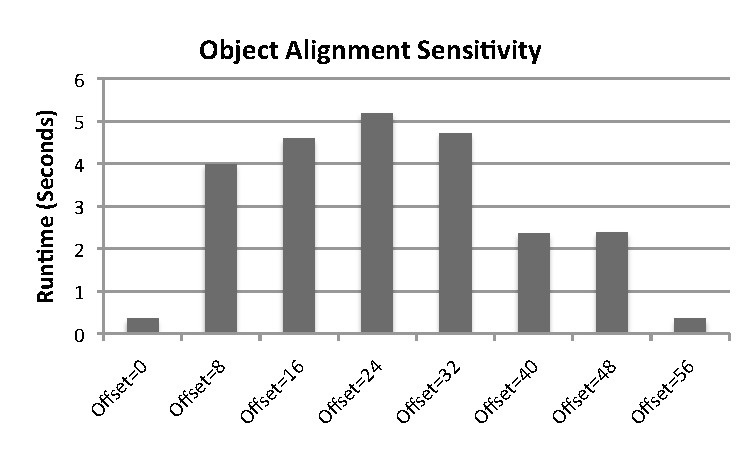
\includegraphics[width=3.3in]{predator/figure/perfsensitive}
\end{center}
\caption{
Performance of the linear\_regression benchmark from the Phoenix benchmark suite.
Performance is highly sensitive to the offset of the starting address of the (potentially) falsely-shared object 
and the start of cache line. 
\label{fig:perfsensitive}}
\end{figure}

The appearance of false sharing depends on 
the alignment between objects and corresponding cache lines.
A real example, linear\_regression, is shown in Figure~\ref{fig:perfsensitive}.
For this benchmark,
when the offset of the starting address between the potentially falsely-shared object and corresponding cache lines 
is $0$ or $56$ bytes, 
there is no false sharing. 
When the offset is $24$ bytes, we see the most severe performance effect caused 
by false sharing. 
The performance difference between these two scenarios can be as large as $15\times$. 
Existing detection tools can only report observed false sharing.
For this case, they may miss a very severe false sharing problem that could occur in the wild if the offset of the starting 
address was $0$ bytes or $56$ bytes in their test environment.
\Predator{} overcomes this shortcoming by accurately predicting potential false sharing.

\begin{figure*}
\begin{center} 
\subfigure[No false sharing]{%
   \label{fig:nofs}
   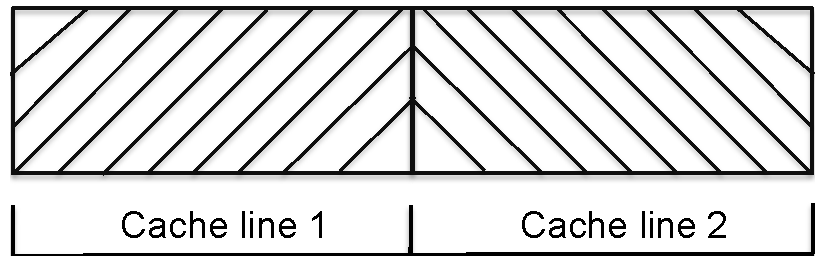
\includegraphics[width=0.24\textwidth]{predator/figure/Potential1}
}%
\hspace{30pt}
\subfigure[False sharing with larger cache size]{%
   \label{fig:fslarger}
   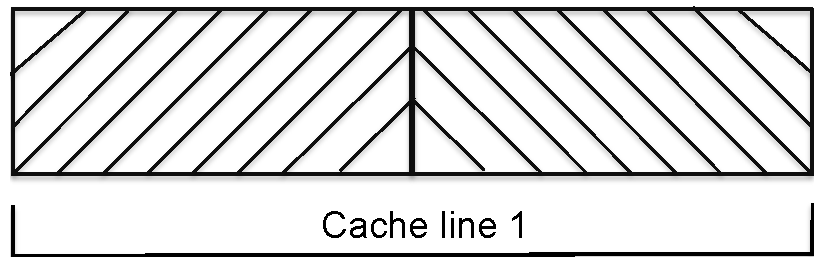
\includegraphics[width=0.24\textwidth]{predator/figure/Potential2}
}%
\hspace{30pt}
\subfigure[False sharing with different alignment]{%
   \label{fig:fsnoalignment}
   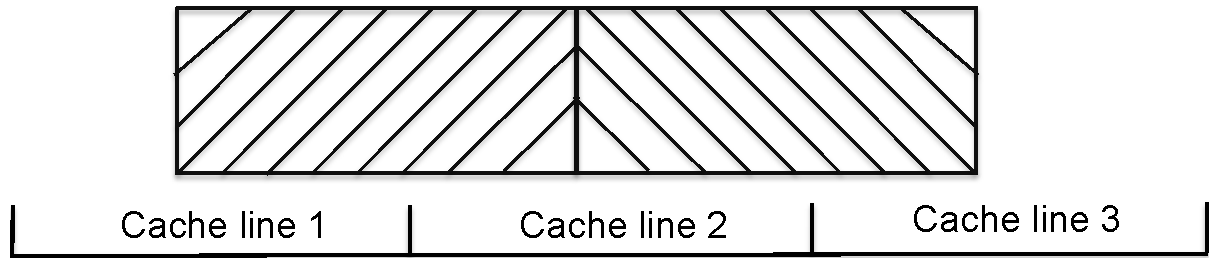
\includegraphics[width=0.36\textwidth]{predator/figure/Potential3}
}%
\end{center}
%\includegraphics{fig/potential.pdf}
\caption{False sharing under different environments.}
\label{fig:potentialfalsesharing}
\end{figure*}

\Predator{} predicts {\it potential false sharing}, the type of
false sharing that does not 
manifest in the current execution but may appear and greatly affect programs' performance
in a slightly different environment.

Figure~\ref{fig:potentialfalsesharing} shows a simplified example why occurrences of false sharing 
can change in different situations.
In this figure, two rectangles with different patterns
represents two portions of the same object, updated by different threads. 
In Figure~\ref{fig:nofs}), there is no false sharing when thread T1 only updates 
``cache line 1'' and T2 only updates ``cache line 2''.
However, false sharing appears in one of the following cases, even with the same
access pattern. 

\begin{itemize}
\item
Doubling cache line size (Figure~\ref{fig:fslarger}). When the size of a
cache line doubles,
both T1 and T2 access the same cache line and false sharing occurs in this case.

\item
Different starting address of an object(Figure~\ref{fig:fsnoalignment}). 
When the starting address of this object is not aligned with the starting address of 
the first cache line, 
then T1 and T2 can update the second cache line simultaneously, 
causing false sharing. 
%When some dynamic property changes the starting address of this object so that it 
%is not aligned with the starting address of the first cache line, 
\end{itemize} 

\Predator{} predicts whether programs can have potential false sharing  
in either of these two cases, where they can be caused by different dynamic properties 
discussed in Section~\ref{sec:intro}.
All dynamic properties, except the change of cache line size,
can lead to different starting address of an object. 
Thus, predicting false sharing in these two cases actually 
explores many possibilities caused by all dynamic properties.

\subsection{Basic Prediction Workflow}
\label{sec:predictionmechanism} 

%Similar to the detection part, 
\Predator{} focuses exclusively on potential false sharing that can 
cause performance problems.
The implementation is based on
two key observations. First, only accesses to 
adjacent cache lines can form potential false sharing, 
i.e., introducing cache invalidations when cache line size
or an object's starting address changes.
Second, only when false sharing introduces a large number of cache invalidations
can it degrade performance.

Based on these two observations, \Predator{} develops 
the following workflow to capture potential false sharing.
Those detection optimizations listed in Section~\ref{optimization} can also be applied
to prediction part. We do not repeat these optimizations in this section.

\begin{enumerate}
\item
Track the number of writes on different cache lines. 

\item
When the number of writes to a cache line $L$ reaches {\it Tracking-Threshold},
track the detailed read and write accesses for every word on both cache line $L$ 
and its adjacent cache lines. 

\item
When the number of writes to a cache line $L$ reaches a second threshold (called as
{\it Predicting-Threshold}), 
identify whether there exists false sharing in $L$ and its adjacent 
cache lines by analyzing word accesses information collected in Step 2. 
Section ~\ref{sec:evaluatingfs} describes the evaluation method.

\item
If a potential false sharing is found, continue to track cache line invalidations to confirm it. Section~\ref{sec:tracking} discusses the details.
Otherwise, go back to Step 2 to track more detailed accesses.
 
\end{enumerate}

\subsection{Searching for Potential False Sharing}
\label{sec:evaluatingfs}
To describe potential false sharing in two different cases, we first 
introduce the concept of a virtual cache line.  A virtual cache line
is a contiguous memory range that spans one or more physical cache 
lines.  In the case of double cache line size, a virtual line is
composed of two original contiguous cache lines and the first cache
line has an even index number.  Thus, only cache lines $2*i$ and
$2*i+1$ can form a virtual line.  In the case of different starting
addresses, a virtual line can have the same size as physical lines,
but can be positioned arbitrarily: unlike actual cache lines, the
starting address of a virtual cache line does not need to be multiple
of the cache line size.  For instance, a 64-byte long virtual line can
consist of the range $[0,64)$ bytes or $[8,72)$ bytes.

To search for potential false sharing problems, 
\Predator{} searches for a hot access pair on $L$ and its adjacent cache lines 
by analyzing the detailed word access information collected in Step 2. 
A hot access in a cache line refers to the word whose number of read or write accesses 
is larger than the average number of accesses to each word of cache line $L$.
For every hot access $X$ in cache line $L$, \Predator{} searches another
hot access $Y$ in $L$'s previous cache line or next cache line satisfying
the following conditions: 

\begin{itemize}
\item
$X$ and $Y$ reside on the same virtual line. 

\item
One of $X$ and $Y$ is a write access.

\item 
$X$ and $Y$ are issued by different threads.

\end{itemize}

% why it finds a pair of $X$ and $Y$ == a potential false sharing 
Whenever it finds such a pair $X$ and $Y$, 
\Predator{} identifies potential performance-degrading false sharing whenever
 the number of cache invalidations caused by $X$ and $Y$, at a possible virtual line, 
is larger than the average number of accesses on each word of $L$. 
This approach is based on a similar observation as in detection:
\emph{if a thread writes a virtual line after other threads 
have accessed the same virtual line, this write operation most likely causes at least one cache 
invalidation}. 
Before tracking detailed memory accesses on a virtual line, it is impossible to know exactly how many cache invalidations happen on a virtual line. Thus, \Predator{} conservatively assumes that accesses from different threads occurs interleavedly.
This approach ensures that \Predator{} does not miss any potential false sharing as well as 
not reporting false positives. 

%According to above observation and assumption, 
%a pair of hot accesses, $X$ and $Y$, if accesses are issued in an interleaving 
%way, can generate the number of cache invalidations equaling to 
%the smaller number of accesses of $X$ and $Y$.
%Thus a false sharing problem is to be identified by \Predator{}.
  
After identifying possible false sharing, \Predator{} goes to Step 4 to 
verify whether this is an actual false sharing problem.

\subsection{Verifying Potential False Sharing}
\label{sec:tracking}

\Predator{} verifies potential false sharing by tracking 
cache invalidations on a problematic virtual line.
%covering a pair of hot accesses found
%in Step 3.

For potential false sharing caused by double cache line size, as described in
Section~\ref{sec:evaluatingfs}, a virtual line is always composed of 
cache line with index $2*i$ and $2*i+1$. 
\Predator{} tracks cache invalidations
on the virtual line on which false sharing has been discovered.

However, for the case of a change in starting address,
two hot accesses with distance less than cache line size 
can form multiple virtual lines. 
There is thus an additional step to determine which virtual line to be tracked.
Although the virtual line to be chosen here is never a real cache line of actual hardware
because of unaligned addresses,
we utilize this virtual line to simulate the effect of changing the 
starting addresses of objects.


\begin{figure}
\begin{center} 
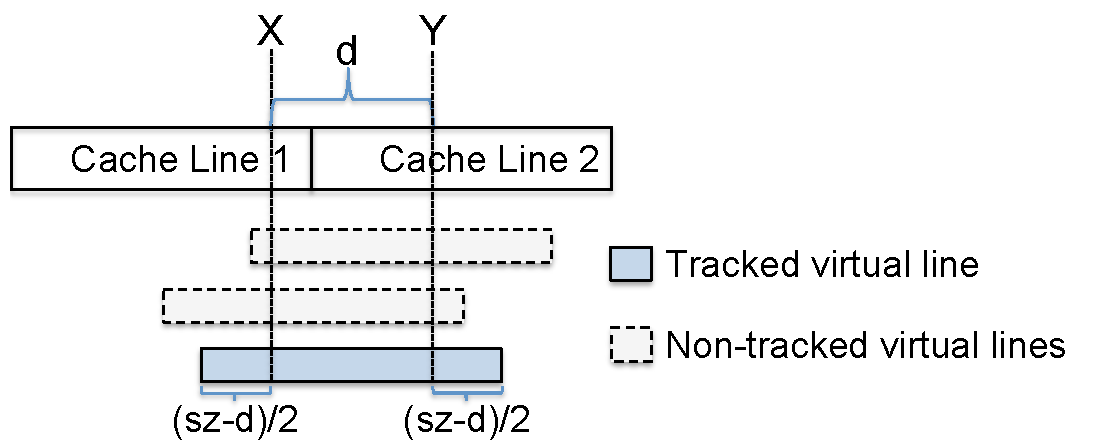
\includegraphics[width=3.3in]{predator/figure/trackpotential}
\end{center}
\caption{Determining a virtual line with size $sz$ according to hot accesses.}
\label{fig:trackpotential}
\end{figure}

Given two words with the hot accesses shown in Figure~\ref{fig:trackpotential}, 
\Predator{} leaves the same space before $X$ and after $Y$ in determining a virtual line. 
That is, the virtual line starting 
at location $X-((sz-d)/2)$ and ending at $Y+((sz-d)/2)$ is tracked. 
This choice allows tracking of more possible cache invalidations caused by
adjacent accesses of $X$ and $Y$. 
Since adjusting the starting address of a virtual line has the same effect of
adjusting the starting address of an object in detecting false sharing,
all cache lines related to the same object must be adjusted at the same time.
\Predator{} then tracks cache invalidations based on these adjusted virtual lines.


%\input{Prediction}

\section{Experimental Evaluation}
\begin{figure*}[htb]
{\centering
\tiny
\subfigure{\lstinputlisting[numbers=none,frame=none,boxpos=t]{predator/figure/linearregression.report}}
\caption{An example report by \Predator{} indicating false sharing in the linear\_regression benchmark.
\label{fig:lrreport}}
}
\end{figure*}



\label{sec:evaluation}

This section answers the following questions:
\begin{itemize}
\item
  How effective is \Predator{} at detecting and predicting false sharing?

\item
  What is \Predator{}'s overhead, in terms of execution time and memory ?

\item
  How sensitive is \Predator{} to different sampling rates?
 
\end{itemize}

\paragraph{Experimental Platform.} All evaluations are performed on a quiescent Intel Core 2 dual-processor system equipped with 
16GB RAM. Each processor is a 4-core 64-bit Intel Xeon running at 2.33 GHz, with a 4MB shared L2 cache and 32KB private L1 cache. The underlying operating system is an unmodified CentOS 5.5, running with Linux kernel version 2.6.18-194.17.1.el5. The glibc version is 2.5. 

\paragraph{Evaluated Applications.}
This paper evaluates two popular benchmark suites,
Phoenix (with large input) ~\cite{phoenix-hpca} and PARSEC (with simlarge input) ~\cite{parsec}. Even with unmodified LLVM-3.2, Facesim cannot be compiled successfully (having complaints on an undefined template) and Canneal aborts unexpectedly. Thus, these two benchmarks are excluded.
We also evaluate \Predator{} on six real applications, including MySQL, Boost, Memcached, aget, pbzip2 and pfscan.



\subsection{Detection and Prediction Effectiveness}
\label{sec:effective}

For every false sharing problem, \Predator{} reports source code information and detailed memory access information in order to help users fix those problems. Figure~\ref{fig:lrreport} shows an example for the linear\_regression benchmark. This report shows that the heap object starting with $0x40000038$ potentially causes a large number of cache invalidations. The call stack of allocation is provided to help locate culprits. In addition, \Predator{} also reports word-level access information of this object, which helps to identify where and how false sharing occurs. From that, we can know that it is a latent false sharing problem predicted by \Predator{}, since different threads are accessing different cache lines. 

\subsubsection{Benchmarks}
\label{sec:benchmarks}

\begin{table*}[!t]
{\centering\begin{tabular}{l|r|r|r|r|r}\hline
{\bf \small Benchmark} & {\bf \small Source Code} & {\bf \small New} & {\bf \small Without Prediction} &{\bf \small With Prediction} & {\bf \small Improvement} \\
\hline
\small \textbf{histogram} & {\small histogram-pthread.c:213} & \cmark{} &\cmark{} & \cmark{} & 46.22\%\\
\small \textbf{linear\_regression} & {\small linear\_regression-pthread.c:133} & & & \cmark{} & 1206.93\% \\
\small \textbf{reverse\_index} & {\small reverseindex-pthread.c:511} & & \cmark{} & \cmark{} & 0.09\%\\
\small \textbf{word\_count} & {\small word\_count-pthread.c:136} & & \cmark{} & \cmark{} & 0.14\%\\
\hline
\small \textbf{streamcluster} & {\small streamcluster.cpp:985} &  & \cmark{} & \cmark{} &7.52\% \\
\small \textbf{streamcluster} & {\small streamcluster.cpp:1907} & \cmark{} & \cmark{} & \cmark{} & 4.77\%\\
\hline
\end{tabular}
\caption{False sharing problems in the Phoenix and PARSEC benchmark suites. \label{table:detection}}
}
\end{table*}

Table~\ref{table:detection} provides detection results of two benchmark suites, Phoenix and PARSEC
The first column lists those programs with false sharing problems.  The second column shows precisely where the problem is. Because all discovered false sharing occurs inside heap objects, we show callsite source code information here.  The third column, ``New'', marks whether this false sharing was newly discovered by \Predator{}.  A checkmark in the following two columns indicates whether the false sharing was identified without
prediction and/or with prediction.  The final column, ``Improvement'', shows the performance improvement after fixing false sharing.
%The number is based on the average runtime of $10$ runs. 

As shown in the table, \Predator{} reveals two unknown false sharing problems. It is the first tool to detect the false sharing problems in histogram and in line $1908$ of streamcluster. 
In histogram, multiple threads simultaneously modify different locations of the same heap object, thread\_arg\_t. 
Padding this data structure fixes the false sharing problem and improves the performance by around 46\%. In streamcluster, multiple threads are simultaneously accessing and updating the same \texttt{bool} array, switch\_membership. Simply changing all elements of this array to a long type reduces the false sharing and improves the performance by about 4.7\%.

%, although it is not a complete fix of false sharing. 
%None of these two false sharing problems has been reported by previous tools.
Other false sharing problems were discovered by previous work~\cite{sheriff}. We do not see significant performance improvement for reverse\_index and word\_count benchmarks. They are reported here because the number of cache invalidations in these two programs reaches our predefined threshold.
Making the reporting threshold higher can avoid the report of those insignificant false sharing problems.
It is worth noting that these two benchmarks definitely have false sharing problems,
which can be confirmed by word-level information generated by \Predator{}. 

The streamcluster benchmark has another false sharing problem at line $985$. Different threads change the work\_mem object simultaneously. Authors of streamclsuter have already realized this problem and provide a CACHE\_LINE macro. Unfortunately, the default value of this macro is set to $32$ bytes, which is different from the actual cache line size of the experimental machine. By setting it to $64$ bytes instead, it achieves  performance improvement of about 7.5\%.

linear\_regression has a severe false sharing problem. Fixing it improves the performance by more than $12\times$. In this benchmark, different threads update their thread-specific locations inside the tid\_args object in a tight loop. According to the observation of Nanavati et al., this false sharing problem occurs when using clang and disappears when using gcc with the -O2 and -O3 optimization level~\cite{OSdetection}. But we observed a different result when using the clang-3.2 compiler and our custom memory allocator: the false sharing problem does not occur at all because the offset of the starting address of the potentially falsely-shared object and the start of cache line is 56 bytes (see Figure~\ref{fig:perfsensitive}). With prediction mechanism, \Predator{} detects this latent false sharing problem, exemplifying the necessity of a predictive detection tool. 

\subsubsection{Real Applications}
To verify \Predator{}'s practicality, we further evaluate several widely-used real applications, whereas no previous work has done this. These real applications include a server application (MySQL~\cite{mysql}),
a standard C++ library (Boost~\cite{libfalsesharing}),
a distributed memory object caching system (Memcached), a network retriever (aget),
a parallel bzip2 file compressor (pbzip2), and a parallel file scanner (pfscan).

MySQL-5.5.32 and boost-1.49.0 are known to have false sharing problems. Other applications (memcached-1.4.15, aget-0.4.1 and pbzip2-1.1.6) do not have known false sharing problems.

The false sharing of MySQL has caused a significant scalability problem and was very difficult to identify.
According to the architect of MySQL, Mikael Ronstrom, ``we had gathered specialists on InnoDB..., participants from MySQL support... and a number of generic specialists on 
computer performance...'', ``[we] were able to improve MySQL performance by 6$\times$ with those scalability fixes''~\cite{mysql}. 
The false sharing inside Boost is caused by the usage of a  spinlock pool. Different threads may utilize different spinlocks located in the same cache line in this case. Fixing it brings a 40\% performance improvement.
\Predator{} is able to pinpoint false sharing locations in both MySQL and the Boost library. 
For the other four applications, \Predator{} does not find severe false sharing problems.

\subsubsection{Prediction Effectiveness}
\label{sec:predicteval}
In this section, we verify whether prediction can always  reveal un-observed false sharing problems.

The linear\_regression benchmark is selected here because of the following two reasons: (1) The false sharing problem of this benchmark cannot be detected without prediction; (2) False sharing severely degrades performance when it actually occurs. Hence, it is a serious problem that should always be detected. 

\begin{figure}[!t]
{\centering
\subfigure{\lstinputlisting[numbers=none,frame=none,boxpos=t]{predator/figure/linearregression.psedocode}}
\caption{The false sharing problem inside the linear\_regression benchmark: multiple threads simultaneously update their entries in lreg\_args.
\label{fig:linearregression}}
}
\end{figure}

Figure~\ref{fig:linearregression} shows the data structure and the source code exercising appropriate false sharing. The size of this data structure, lreg\_args, is $64$ bytes 
when the program is compiled to a $64$-bit binary. For this benchmark, the main thread allocates an array, containing as many elements as the number of underlying hardware cores. Each element is a lreg\_args type with $64$ bytes. This array is then passed to different threads (lreg\_thread function) so that each thread only updates its thread-dependent area. False sharing occurs if two threads happen to update data in the same cache line. 

Figure~\ref{fig:perfsensitive} shows how sensitive the performance is to different starting addresses of a falsely-shared object. When the offset is $0$ or $56$ bytes, this benchmark achieves its optimal performance and has no false sharing. When the offset is $24$ bytes, the benchmark runs around $15$ times slower than its optimal performance because of the false sharing problem.

Our evaluation shows that \Predator{} can always detect the false sharing problem with prediction enabled, demonstrating its effectiveness.

\subsection{Performance Overhead}
\label{sec:perfoverhead}

\begin{figure*}[!t]
\centering
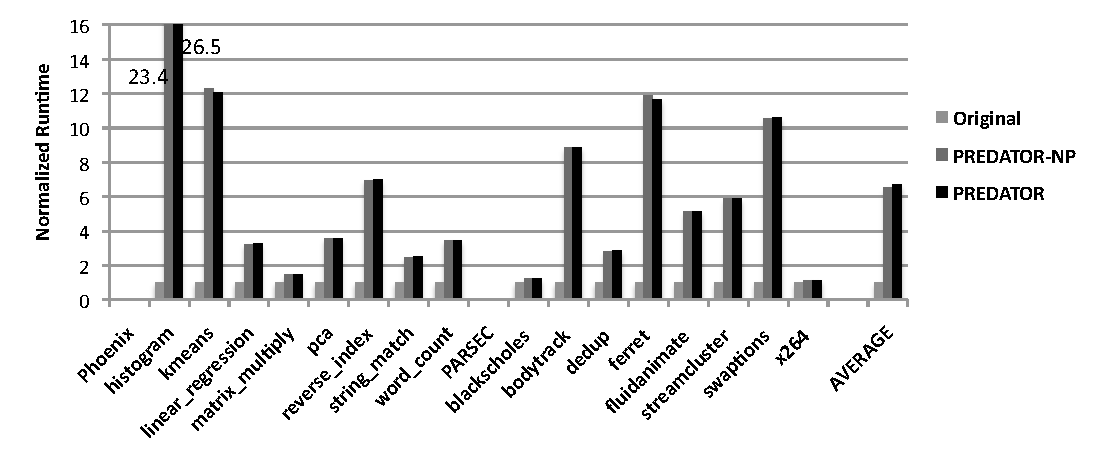
\includegraphics[width=6in]{predator/figure/perf}
\caption{
Performance overhead of \Predator{} with and without prediction(PREDATOR-NP).
\label{fig:perf}}
\end{figure*}

To avoid the effect caused by extreme outliers, all performance data shown in Figure~\ref{fig:perf} is based on the average of $10$ runs, excluding the maximum and minimum values. 

For $16$ benchmarks from the Phoenix and PARSEC benchmark suites and six real applications, \Predator{} imposes $5.4\times$ performance overhead. There is no noticeable difference on performance whether the prediction mechanism is enabled or not. 
 
Among these programs, five of them, histogram, kmeans, bodytrack, ferret, and swaptions, have more than $8\times$ performance overhead. The histogram benchmark runs more than $26\times$ slower than original executions with \pthreads{} library, because tracking detailed access on cache lines with false sharing exacerbates the false sharing effect (see more discussion in Section~\ref{sec:sample}).  For bodytrack and ferret, although there is no false sharing, \Predator{} detects a large amount of cache lines with writes larger than {\it Tracking-Threshold}. Thus, tracking those accessing details for those cache lines imposes significant performance overhead. Currently, we cannot identify the reasons why kmeans runs very slowly on \Predator{}.
   
\Predator{} imposes a small performance overhead for IO-bound applications, such as matrix\_multiply, blackscholes, x264, aget, Memcached, pbzip2, and pfscan, since \Predator{} does not add any performance overhead for IO operations.  

\subsection{Memory Overhead}
\label{sec:memoverhead}
We only evaluate the physical memory overhead of \Predator{}, instead of the virtual memory overhead, because \Predator{} allocates four gigabytes virtual memory for its custom memory allocator. Proportional set size (PSS) in \texttt{/proc/self/smaps} reflects the physical memory increase on the existing system of running an application~\cite{memusage}. Thus, we periodically collect this data and use the sum of different memory mappings as the total physical memory usage of running an application. We present the maximum value of physical memory usage in Figure~\ref{fig:memusage}. 

\Predator{} imposes less than 50\% memory overhead for 17 out of 22 applications.  For swaptions and aget, \Predator{} introduces more memory overhead because the original memory footprints of them are very small, only $3$ kilobytes. Adding the code of detection, prediction and reporting contributes to a large ratio of memory overhead. We are not clear why MySQL consumes much more memory than others. Although the average memory usage of all applications is over $2\times$, the total memory usage overhead is only about $40\%$ on \Predator{}. 


\subsection{Sensitivity to Different Sampling Rates}
\label{sec:sensitivity}
In Section~\ref{sec:sample}, we discuss that \Predator{} utilizes the sampling mechanism to reduce the tracking overhead. Running an application with different sampling rates does not affect its memory usage. Thus, we only evaluate the effect of different sampling rates on performance and effectiveness. 

The default sampling rate used by \Predator{} is 1\%. In this section, we also evaluate two other sampling rates, 0.1\% and 10\%. The performance results under the three different sample rates are shown in Figure~\ref{predator/figure:sample}. \Predator{} introduces less performance overhead under a lower sampling rate, which meets our expectation. Concerning effectiveness, even using the 0.1\% sampling rate, \Predator{} can still detect all false sharing problems, but with a lower number of cache invalidations. Thus, different sampling rates do not affect the detection effectiveness.
 
\begin{figure*}[!t]
\centering
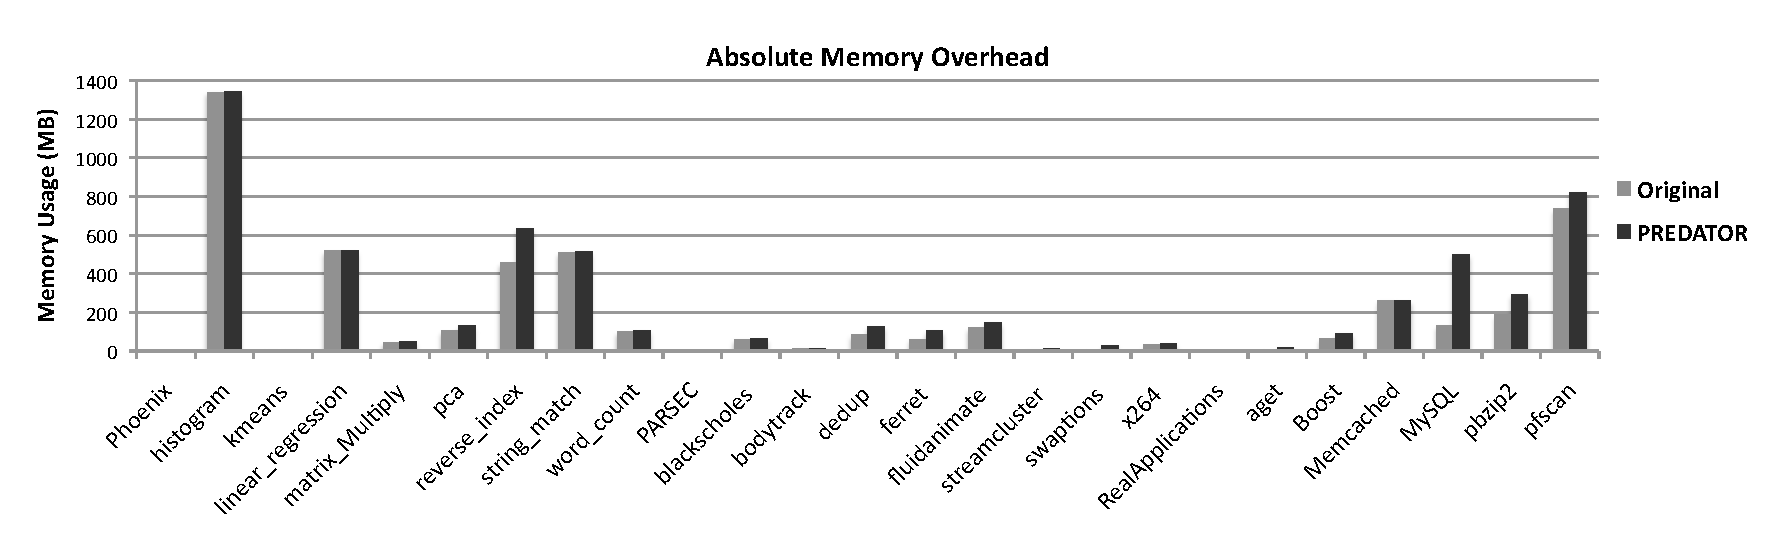
\includegraphics[width=6in]{predator/figure/absolutememory}
\caption{Absolute physical memory usage overhead with \Predator{}.}
\label{fig:absolutememusage}
\end{figure*}

\begin{figure*}[!t]
\centering
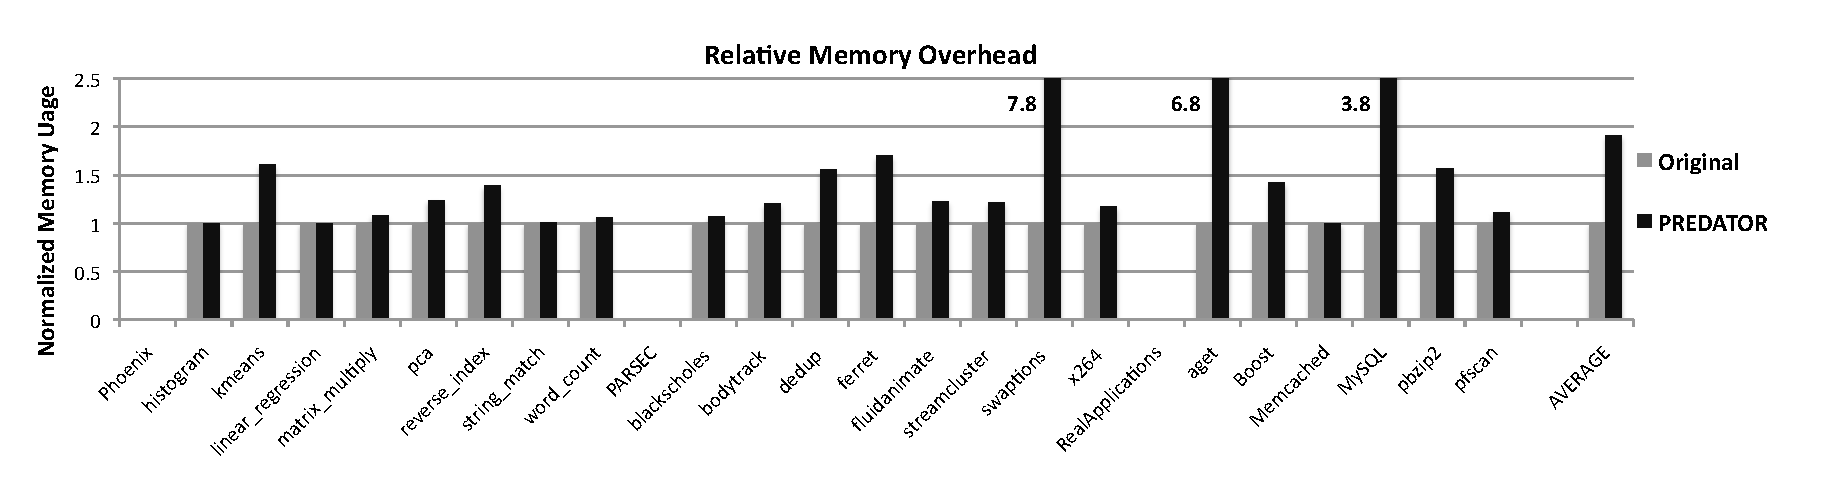
\includegraphics[width=6in]{predator/figure/memusage}
\caption{Relative physical memory usage overhead with \Predator{}.}
\label{fig:memusage}
\end{figure*}



\section{Limitation and Future Work}
\label{sec:discussion}

\subsection{Instrumentation Selection}
\label{sec:instrumentationtradeoff}
Dynamic binary instrumentation and compiler-based instrumentation are two alternative approaches to perform instrumentation~\cite{Instrumentation}. They exhibit different tradeoffs of performance and generality. Dynamic binary instrumentors, such as Valgrind~\cite{Valgrind}, Pin~\cite{Pin}, and DynamoRIO~\cite{DynamoRIO}, typically analyze the program's code just before execution in order to insert instrumentation. They introduce significant performance overhead, mostly caused by run-time encoding and decoding, but the fact that they operate directly on binaries makes them extremely convenient. By contrast, compiler instrumentation inserts instrumentation in the compilation phase, which requires re-compilation of all source code. 
\Predator{} employs compiler-based instrumentation both because of its better performance and its greater flexibility, as discussed in Section~\ref{sec:selectinstrumentation}.

\subsection{Effectiveness}
Several factors can affect \Predator{}'s ability to identify false sharing.

\emph{Different Inputs.} Different inputs trigger distinct executions of a program. If a specific input does not exercise the code with false sharing problems, \Predator{} cannot necessarily detect them. However, \Predator{} does generalize over inputs to find latent false sharing problems on those exercised code. When any reasonably representative set of inputs are exercised, as is required by any testing regime, \Predator{} can effectively predict false sharing.

\emph{Input Size.} Input size may affect detection results.  As discussed in Section~\ref{optimization}, \Predator{} introduces several threshold values to reduce tracking overhead, which can be adjusted as needed. If the input size is so small that it cannot generate enough false sharing events to cross the pre-defined thresholds, then the detection mechanism will not be triggered. In such cases, \Predator{} will miss actual cases of false sharing. However, realistically large inputs should be enough to trigger \Predator{}'s detection mechanisms. 

\emph{Hardware Independence.}  \Predator{}'s compiler-based approach make it independent of the underlying hardware platform. This approach increases generality, but may lead to over-report false sharing. \Predator{} conservatively assumes that different threads are running on different cores and detects false sharing problems based on possible cache invalidations. However, if multiple threads involved in false sharing are on the same core, then there will be no performance impact. 

%\subsection{Prediction Limitations} 
%\Predator{} can accurately and precisely predict a false sharing problem even when it does not occur. But \Predator{} cannot predict a false sharing problem if the code with false sharing is not exercised at all. Also, \Predator{} may miss potential false sharing problems between two objects brought by a different compiler or memory allocator. 


%\section{Issues}
%(1) Maybe user should have a option to check those false sharing inside stack variables.
(2) Should we use a thread index instead to save some spaces? Also, maybe it is better for the performance. 
    Generally, we will not have two threads that are accessing the same subheap. However, we may have to use
    the pthread\_t for comparison since it is unique? but actually it is not.
    We should use the unique heap in order to avoid the lock usage and overlapping (Diehard problem). In Diehard,
    two threads can use the same heap every time. 
    Also, we may introduce the current pointer in the thread library so that we can know corresponding information quickly. 
    whenever all children threads has been exited, then we should possibly update the 
    So we should use a

(3) Should we have an internal heap which also use tid to index their subheap.
(4) When there are multiple files there, how we can instrument every file one by one? Design a makefile to do this automatically. 

(a) Inserting the into clang so that we do not need to change the make file for each files.
(b) We will keep track of each read/write accesses instead of only checking once for each basic block.


Improving the performance step by step
(1) Avoiding using the singleton if we can use the simple variable.
(2) Trying to use the sampling (100 instructions we only sample one).

(4) How to sample those accesses. We donot want to loose those cache invalidations. 
So for each cache line, we are using the cache line based sampling mechanism. 
In the non-sampling phase, we will not update everything. 

However, there is a per-thread based sampling. For example, we only sample those accesses in the 
first 500 over 1000 accesses. However, we may lost a lot of interleaving accesses by doing this. 

If we are using the system level accessCount, for example, updating this shared accesses can cause a lot of
invalidations - which cause a lot of performance problem by using the shared account.

Also, we should try to implement those very basic accesses incremental in the first level instead of inside a very deep level.



\section{Related Work}

\label{chapter:relatedwork}
This chapter first describes those related work to processes-as-threads framework and deterministic execution. Then it describes related work in false sharing detection, prevention, or both. 

\section{Processes-As-Threads framework}

BOP relies on strong isolation of processes to automatically and safely parallelize the execution of programs~\cite{DingBOP}. BOP forks a new process to do speculation, based on those pre-defined possibly parallel regions (PPR). In order to check the correctness, BOP tracks accesses on a page-based granularity. When there is no conflict and a speculative process reaches the end of its current PPR, its predecessor always commits its changes to the current process. However, BOP does not provide any synchronization support and can not be used to run normal multithreaded programs. 

Grace is a process-based approach designed to prevent
concurrency errors, such as deadlock, race conditions, and
atomicity errors by imposing a sequential semantics on
speculatively-executed threads~\cite{grace}. Grace supports only fork-join programs without inter-thread communication (e.g., condition variables or barriers), and rolls back threads when accesses of threads would violate sequential semantics: a thread accesses pages that have been accessed by its predecessors. Grace can not support arbitrary multithreaded programs. Similar to the Grace system, Sammati is a processes-as-threads system to detect and tolerate deadlock problems~\cite{Pyla:2010:ADA:1854273.1854288}. However, Sammati does not support the full range of synchronizations, without synchronizations, barriers, and signals. Also, Semmati can not avoid race conditions happening in creating twin pages, which are avoided by \Sheriff{} framework.

\begin{comment}
% Some usage of this framework
According to Revisions,  Grace cannot easily resolve all
conflicts on commit (like revisions do) and must thus restrict
tasks from producing such conflicts either statically (by type
system) or dynamically (pessimistic with blocking, or optimistic with abort and retry). Also, Grace allows only a restricted “fork-join” form of concurrency
Revisions~\ref{Burckhardt:2010:CPR:1869459.1869515}
\end{comment}

\section{Deterministic Multithreading}
The research on deterministic multithreading is a very active area these years. We describe some software-only, non- language-based approaches here.

\subsection{Software-only deterministic system}
Grace prevents deadlocks, race conditions, ordering and atomicity violations errors for those fork-join multithreaded programs by imposing a sequential semantics at join points~\cite{grace}. However, Grace does not support programs with interthread communications, such as conditional variables and barriers.

CoreDet is a compiler-based approach to 
support general-purpose multithreaded programs~\cite{Bergan:2010:CCR:1736020.1736029}. 
CoreDet instruments those memory read and write operations as long
as those operations can not be proved to be thread-local in static analysis. 
In the runtime phase, CoreDet divides the execution into 
alternating parallel and serial phases and guides all memory operations 
using a memory ownership table: only those owned locations can be accessed
in the parallel phases; all non-owned locations and synchronizations can only 
be accessed in the serial phases guided by a global token.
CoreDet guarantees deterministic execution for racy programs without memory errors,
but with very high performance overhead: 
averagely $3.5\times$ slower than those using \pthreads{} library.
In order to guarantee determinsim, 
CoreDet has to serialize \emph{all} external library calls without instrumentation.
CoreDet doesn not provide deterministic 
memory allocations, which can not guarantee determinism for programs with memory errors.  
% The use of synchronization points as commit boundaries also makes \dthreads{}
% code relatively \emph{robust}: when updates occur after a given number of 
% instructions retired (as in CoreDet and Kendo), it is impossible for 
% programmers to know when interleavings can occur. Such boundaries could vary 
% depending on the underlying architecture and would also be input-dependent, 
% meaning that slightly different inputs could lead to dramatically different
% thread interleavings. By contrast, \dthreads{} guarantees that only changes to
% the sequence of synchronization operations affect the order in which updates 
% are applied.
dOS~\cite{deterministic-process-groups} is an extension to CoreDet
that uses the same deterministic scheduling framework.  dOS 
supports deterministic communication for those threads and processes inside the same
deterministic process groups (DPGs) and handle those external non-determinism by recording and
replaying interactions across DPG boundaries. 

Determinator is a microkernel-based operating system that enforces
system-wide determinism~\cite{efficient-system-enforced}.
Determinator provides separate address spaces and supports interprocess
communications at explicit synchronizaton points. 
Determinator is a proof-of-concept system, which can not support the whole rage of
threads APIs and can not work on legacy programs.  

Some other works can only support limited determinism or need user annotation.
Kendo can only guarantee the determinism for race-free programs~\cite{1508256}. 
TERN~\cite{stable-deterministic} provides a best-effort system to 
apply memoized schedules for future runs with similar inputs. 
It can not guarantee the determinism for racy programs, as Kendo. 
Peregrine~\cite{peregrine:sosp11} is a system based on TERN, which tries to record
 memory accesses orders for racy portion and apply those schedules for future runs possibly.
However, both TERN and Peregrine do not support complete determinism (using a best effort)
and requires program annotations. 

\subsection{Hardware-related deterministic System}

\section{False Sharing}

This section describes related work in false sharing detection, prevention, or both. There is no previous
system to predict unobserved false sharing.

\subsection{False Sharing Detection}
Based on the SIMICS functional simulator, Schindewolf et al.\ designed a tool to report different kinds of cache usage information, such as cache misses and cache invalidations~\cite{falseshare:simulator}. Pluto relies on Valgrind dynamic instrumentation framework to track the sequence of memory read and write events on different threads, and reports a worst-case estimation of possible false sharing~\cite{falseshare:binaryinstrumentation1}.
Similarly, Liu uses Pin to collect memory access information, and reports total cache miss information~\cite{falseshare:binaryinstrumentation2}.
These tools impose about $100-200\times$ performance overhead.

Zhao et al.\ developed a tool based on DynamoRIO framework to detect false sharing and other cache contention problems
for multithreading programs~\cite{qinzhao}. 
It uses a shadow memory technique to maintain memory access history and detects cache invalidations based on the ownership of cache lines. However, it can only support at most $8$ threads. In addition, it cannot differentiate cold cache misses from actual false sharing problems.

Intel's performance tuning utility (PTU) uses Precise Event Based Sampling (PEBS) hardware support to detect false sharing problems ~\cite{detect:ptu, detect:intel}.  PTU cannot distinguish true sharing from false sharing. In addition, PTU aggregates memory accesses without considering memory reuses and access interleaving, leading to numerous false positives. Sanath et al. designed a machine learning based approach to detect false sharing problems. They train their classifier on mini-programs and apply this classifier to general programs ~\cite{mldetect}. Instead of instrumenting memory accesses, this tool relies on hardware performance counters to collect memory accesses events. It achieves very low performance overhead(about 2\%). But it relies on hardware support for its efficiency.  

In addition to their individual disadvantages,
all approaches discussed above share a common shortcoming:  
they cannot pinpoint the exact location of false sharing in the source code, so programmers have to examine the source code and identify problems manually.

Pesterev et al.\ present DProf, a tool that help programmers identify cache misses based on AMD's instruction-based sampling hardware~\cite{DProf}. DProf requires manual annotation to locate data types and object fields, and cannot detect false sharing when multiple objects reside on the same cache line.

\subsection{False Sharing Prevention}
\label{sec:fspreventwork}
% More approaches
Jeremiassen and Eggers use a compiler transformation to automatically adjust the memory layout of applications through padding and alignment~\cite{falseshare:compile}. Chow et al.\ alter parallel loop scheduling in order to avoid false
sharing~\cite{falseshare:schedule}. These approaches only works for regular, array-based scientific code.

Berger et al.\ describe Hoard, a scalable memory allocator that can reduce the possibility of false sharing by making different threads use different heaps~\cite{Hoard}. Hoard cannot avoid false sharing problem in global variables or within
a single heap object: the latter appears to be the primary source of real false sharing problems.

\subsection{False Sharing Detection and Prevention}

Plastic leverages the sub-page granularity memory remapping facility provided by the Xen hypervisor to detect and tolerate false sharing automatically~\cite{OSdetection}. However, the sub-page memory remapping mechanism is not currently supported by most existing operating system, reducing its generality. In addition, Plastic cannot pinpoint the exact source of false sharing.  
In order to utilize Plastic's prevention tool, a program has to run on the Xen hypervisor, limiting the applicability of their prevention technique.



\section{Conclusion}
\label{sec:conclusion}

\dthreads{} is a deterministic replacement for the \pthreads{}
library that supports general-purpose multithreaded
applications. \dthreads{} is straightforward to deploy, requiring no
source code, and operates on commodity hardware. By converting threads
into processes, \dthreads{} leverages process isolation and virtual
memory protection to track and isolate concurrent memory updates with
low overhead. By committing these changes deterministically at natural
synchronization points in the code, rather than at boundaries based on
hardware performance counters, \dthreads{} not only ensures full
internal determinism---eliminating data races as well as
deadlocks---but does so in a way that is portable and easy to
understand. Its software architecture prevents false sharing, a
notorious performance problem for multithreaded applications running
on multiple, cache-coherent processors. The combination of these
approaches enables \dthreads{} to match or even exceed the performance
of \pthreads{} for the majority of the benchmarks examined here,
making \dthreads{} a safe and efficient alternative to \pthreads{} for
some applications.


%\section{Acknowledgement}
%\acks
%\input{acknowledge}

%\appendix
%\section{Manual}

%\section{How to Integrate with LLVM}





% We recommend abbrvnat bibliography style.

%\bibliographystyle{abbrvnat}

% The bibliography should be embedded for final submission.
{
\bibliographystyle{abbrv}
\bibliography{refs}
}

%\begin{thebibliography}{}
%\end{thebibliography}

\end{document}
